\chapter{Серьёзные испытания}


\setlength{\epigraphwidth}{.80\textwidth}
\epigraph{Со временем разум поднимется на более высокий уровень знаний, но не сможет понять, как он там оказался.
%There comes a time when the mind takes a higher plane of knowledge but can never prove how it got there.
}{--- Альберт Эйнштейн (1879---1955)}

Ну да, как будто предыдущие головоломки не были сложными, а тут ещё несколько непростых задач.
Хотя может случиться, что некоторые из них покажутся проще.
Ведь то, что ставит одного в тупик, бывает легко другому.


\subsection*{Торт-мороженое}\label{Торт-мороженое}

На столе стоит цилиндрический торт-мороженое сверху покрытый шоколадной глазурью.
Мы последовательно отрезаем от него дольки с углом $x$, где $x$ произвольно,
каждый раз долька переворачивается и вставляется обратно в торт
(рис. \ref{pic:tort}).

Докажите, что после конечного числа таких операций вся глазурь снова окажется сверху!


\begin{figure}[htb!]
\centering
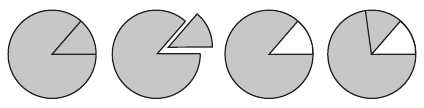
\includegraphics[scale=1]{pics/tort}
\caption{Разрез, переворот, и снова разрез.}
\label{pic:tort}
\end{figure}

\parit{Примечание.}
Я называю такие задачи \emph{вроде неверно расслышанные}.
Да-да, угол $x$ может быть иррациональным. 
В этом случае вы никогда не отрежете одинаковый кусок дважды.
Придётся отрезать довольно много долек, но всё же конечное число.
К счастью, торт-мороженое самовосстанавливается.

\subsection*{Прыгание и перепрыгивание}

Лягушка прыгает по длинной цепочке кувшинок;
на каждой кувшинке она подбрасывает монету, чтобы решить,
сделать ли двойной прыжок вперёд или же одинарный назад.
На какой доле кувшинок она побывает?

\subsection*{Три тени кривой}\label{Три тени кривой}

Существует ли простая замкнутая кривая в трёхмерном пространстве, все три проекции которой на координатные плоскости являются деревьями?

\parit{Примечание.}
Это означает, что тени кривой в трёх координатных направлениях не содержат циклов.
На рис. \ref{pic:proj1} изображена кривая, которая почти подходит: две её тени являются деревьями, но третья содержит (и даже является) циклом.

\begin{figure}[htb!]
\centering
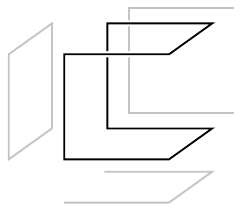
\includegraphics[scale=1]{pics/proj1}
\caption{Замкнутая кривая у которой пара проекций деревья.}
\label{pic:proj1}
\end{figure}

\subsection*{Игроки и победители}

Тристану и Изольде предстоит очутиться в ситуации с очень ограниченной связью, в которой Тристан будет знать, какие две из 16 баскетбольных команд сыграли матч, а Изольда узнает, кто выиграл.
Сколько битов необходимо передать им друг другу, чтобы Тристан узнал, кто одержал победу?

\parit{Примечание.}
Эта задача по \emph{коммуникационной сложности}.
Если бы Изольда знала, кто играл, а также кто выиграл, она могла бы отправить один бит, чтобы сообщить Тристану, выиграла ли (скажем) команда, идущая первой по алфавиту.
Без этой информации она могла бы просто отправить четыре бита, чтобы определить победившую команду.
А можно ли обойтись меньшим числом битов?

\medskip

А вот ещё задача по коммуникационной сложности, но посложней.

\subsection*{Подсказка для Чарли}

Алиса и Боб знают да-нет ответы на все $n$ вопросов экзамена, который сдаёт Чарли.
Чарли нужен только ответ на $k$-й вопрос, но ни Алиса, ни Боб не знают значение $k$.
Вместо этого Алиса знает число $i$, Боб --- число $j$, такие, что $k = i + j \pmod n$.
При этом Чарли знает оба числа $i$ и $j$.

Если бы Алиса не могла передать никакой информации,
то Бобу пришлось бы отправить Чарли все ответы (всего $n$ битов), чтобы Чарли смог узнать нужный ему ответ.

Докажите, что если Чарли получит всего один бит от Алисы, то Бобу достаточно отправить всего $n/2$ битов.

\subsection*{Сближение по кривой}

\begin{figure}[htb!]
\centering
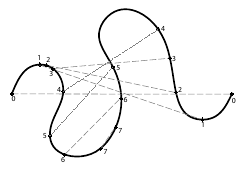
\includegraphics[scale=1]{pics/s-curve}
\caption{Кривая с обоими свойствами.}
\label{pic:s-curv}
\end{figure}

Плоская кривая на рис. \ref{pic:s-curv} обладает следующими свойствами:
(1) расстояние между её конечными точками больше, чем у любой другой пары точек на кривой (мы используем обычное евклидово расстояние на плоскости),
и
(2) взяв по карандашу в обе руки, можно поставить их кончики в концах кривой и двигать их вдоль кривой до встречи, так, чтобы \emph{в процессе расстояние между ними не увеличивалось}.

Существует ли кривая со свойством (1), но без свойства (2)?


\subsection*{Суммы и произведения}

В шляпе лежат все целые числа, большие 1, но меньшие 100.
Из неё достают два числа.
Саманта узнаёт их сумму, а Порфирио --- их произведение.
Далее, Саманта говорит:

--- Я знаю, что ты не знаешь этих чисел.

--- Теперь я их знаю, --- отвечает Порфирио.

--- Теперь и я знаю, --- говорит Саманта.

Что это были за числа?

\begin{figure}[htb!]
\centering
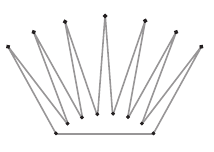
\includegraphics[scale=.95]{pics/korona}
\caption{Корона.}
\label{pic:korona}
\end{figure}

\begin{figure}[htb!]
\centering
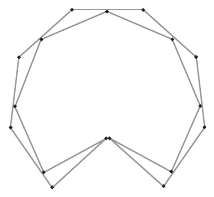
\includegraphics[scale=.95]{pics/wreath}
\caption{Венок.}
\label{pic:wreath}
\end{figure}

\begin{figure}[htb!]
\centering
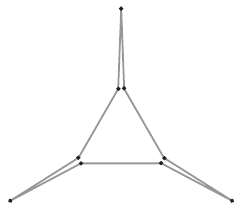
\includegraphics[scale=.95]{pics/treug}
\caption{Схлопнутый треугольник.}
\label{pic:treug}
\end{figure}

\subsection*{Сложенный многоугольник}\label{Сложенный многоугольник}

Какова минимальная площадь простого многоугольника с нечётным числом сторон, каждая из которых имеет единичную длину?

\parit{Примечание.}
Простой многоугольник это замкнутая ломаная без самопересечений, состоящая из конечного числа звеньев.
Многоугольник не обязан быть выпуклым,
например, он может выглядеть как один из многоугольников на рис. \ref{pic:korona},
\ref{pic:wreath} и \ref{pic:treug}.
Очевидно, что у многоугольника на рисунке \ref{pic:treug} площадь не менее площади равностороннего треугольника с единичными сторонами, то есть $\sqrt{3}/4$.
Несложно проверить, что и площадь короны на рис. \ref{pic:korona} ограничена тем же числом.
Но про венок на рис. \ref{pic:wreath} это уже не так очевидно.

Равносторонние \emph{чётно}угольники могут иметь произвольно малую площадь, например, складываясь в очень остроконечную звезду.
А что по поводу нечётноугольников --- могут ли они иметь площадь меньше $\sqrt{3}/4$?
Попробуйте это доказать или опровергнуть?

